\subsection{Разработка архитектуры программного средства}
\label{sec:design:architecture}

Классической архитектурой для мобильных приложений является двузвенная клиент-серверная архитектура. В простейшем случае единственная задача сервера -- возврат по запросу статической страницы с некоторой информацией. Однако в настоящее время данный подход устарел и используется в крайне простых приложениях: в основном для информационных сайтов~\cite{from_sites_to_webapps}. Абсолютное большинство ресурсов сети Интернет реализованы с высокой степенью интерактивности, то есть предоставляют некоторые элементы, с которыми пользователь может взаимодействовать. Таким образом, клиентская часть приложения, помимо простого отображения информации, должна быть управляемой с помощью пользовательских воздействий. Выбранная в пункте \ref{sec:analysis:specification:language} программная платформа позволяет нам это реализовать.

Вследствие интерактивности появляется необходимость в хранилище\linebreakданных, которая обычно решается с помощью реляционных баз данных. В пункте \ref{sec:analysis:specification:language} указано, что в приложении будет использоваться MongoDB, которая может запускаться на физически отдельной ЭВМ. Таким образом, приходим к трехзвенной архитектуре, схема которой представлена на рисунке~\ref{fig:analysis:specification:language:3-tier}.

\begin{figure}[ht]
\centering
	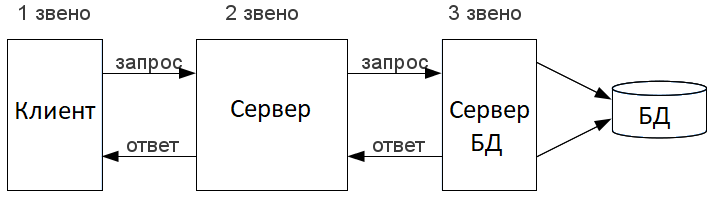
\includegraphics[scale=0.85]{3-tier.png}
	\caption{Вариант трехзвенной архитектуры}
	\label{fig:analysis:specification:language:3-tier}
\end{figure}

Появляется вопрос о необходимости серверной части приложения. Клиентская часть с помощью, например, протокола HTTP может сама без промежуточных звеньев обращаться к базе данных. Однако от данной модификации архитектуры было решено отказаться, поскольку появлются существенные риски нарушения требований безопасности: потребовалось бы наличие открытого API для взаимодействия клиента с БД, которое могло бы легко использоваться злоумышленником. В нашем случае серверная часть реализует так называе <<middleware>> (промежуточные звенья). При любом запросе со стороны клиентской части серверная, прежде чем выполнить дейтвие, индентифицирует пользователя, с устройства которого был отправлен запрос. Если токен пользователя совпадает с токеном, хранящимся на сервере, то происходит дальнейшее выполнение запроса. В противном случае возращается ответ с ошибкой.
